\documentclass[aspectratio=169]{beamer}

% <<< BEGIN tema

\usetheme[nomyriadpro]{unam}

% logos (los valores por defecto ya apuntan a assets/; se pueden cambiar aquí)
\unammotto{}
\unamslidelogo{
\includegraphics[width=0.45\paperheight]{assets/unam-escudo-gris}}

% sin símbolos de navegación
\beamertemplatenavigationsymbolsempty

% cómo se muestran los elementos ocultos: invisible / transparent / dynamic
\setbeamercovered{transparent}
\setbeamersize{text margin left=1.2em,text margin right=1.2em}
\addtobeamertemplate{frametitle}{}{\vspace{0.2em}}

% >>> END

% <<< BEGIN paquetes y macros

\usepackage{amsmath,amssymb,mathtools}
\usepackage{physics}
\usepackage{bm}
\usepackage{booktabs}
\usepackage{xcolor}
\usepackage{hyperref}
\usepackage[utf8]{inputenc}
\usepackage[T1]{fontenc}
\DeclareFontShape{T1}{cmss}{b}{n}{<->ssub*cmss/bx/n}{}
\DeclareFontShape{T1}{cmss}{m}{sc}{<->ssub*cmr/m/sc}{}

% gráficos con TikZ
\usepackage{tikz}
\usetikzlibrary{fit, backgrounds, arrows.meta, positioning}

% carpeta de imágenes
\graphicspath{{images/}}

\definecolor{myblue}{RGB}{30,100,180}
\definecolor{myred}{RGB}{180,30,30}
\definecolor{mygreen}{RGB}{20,140,60}
\definecolor{mypurple}{RGB}{120,30,160}
\definecolor{myorange}{RGB}{220,120,0}

% macros de ejemplo (agregar las propias del proyecto aquí)
\newcommand{\kv}{\mathbf{k}}
\newcommand{\etal}{\textit{et al.}}

% >>> END

% <<< BEGIN metadatos

\title[Título corto]{Título de la presentación}
\subtitle[Subtítulo corto]{Subtítulo de la presentación}
\author[Autor]{Nombre del autor}
\institute{Universidad Nacional Autónoma de México}
\date{Noviembre 2026}
\venue{Universidad Nacional Autónoma de México}

% >>> END

\begin{document}

\titleframe

% ====================================================
\section{Elementos del template}
% ====================================================

% ---- listas ----
\begin{frame}{Listas}
  \begin{columns}[T]
    \begin{column}{0.48\textwidth}
      \textbf{Itemize}
      \begin{itemize}
        \item Primer nivel.
          \begin{itemize}
            \item Segundo nivel.
              \begin{itemize}
                \item Tercer nivel.
              \end{itemize}
          \end{itemize}
        \item Texto con \alert{alert} y \emph{énfasis}.
      \end{itemize}
    \end{column}
    \begin{column}{0.48\textwidth}
      \textbf{Enumerate}
      \begin{enumerate}
        \item Primer paso.
        \item Segundo paso.
        \item Tercer paso.
      \end{enumerate}
      \vspace{0.5em}
      \textbf{Description}
      \begin{description}
        \item[PT] Teoría de perturbaciones.
        \item[EFT] Teoría efectiva de campos.
      \end{description}
    \end{column}
  \end{columns}
\end{frame}

% ---- bloques ----
\begin{frame}{Bloques}
  \begin{block}{Block}
    Bloque estándar para resaltar una idea.
  \end{block}
  \vspace{0.5em}
  \begin{alertblock}{Alert block}
    Bloque para advertencias o puntos clave.
  \end{alertblock}
  \vspace{0.5em}
  \begin{exampleblock}{Example block}
    Bloque para ejemplos.
  \end{exampleblock}
\end{frame}

% ---- ecuaciones ----
\begin{frame}{Ecuaciones}
  \textbf{Ecuación destacada:}
  \[
    P(k) = \int \dd^3 r \; \xi(r)\, e^{-i\kv\cdot\mathbf{r}}
  \]
  \textbf{Ecuaciones alineadas:}
  \begin{align*}
    \delta(\kv) &= \delta^{(1)}(\kv) + \delta^{(2)}(\kv) + \dots \\
    \langle \delta(\kv)\,\delta(\kv') \rangle &= (2\pi)^3\, \delta_D(\kv+\kv')\, P(k)
  \end{align*}
\end{frame}

% ---- columnas + figura ----
\begin{frame}{Columnas con figura}
  \begin{columns}[c]
    \begin{column}{0.48\textwidth}
      Las imágenes van en la carpeta \texttt{images/} y se incluyen con
      \begin{itemize}
        \item \texttt{\textbackslash includegraphics\{nombre\}}
      \end{itemize}
    \end{column}
    \begin{column}{0.48\textwidth}
      \centering
      % reemplazar por: \includegraphics[width=\linewidth]{mi-figura}
      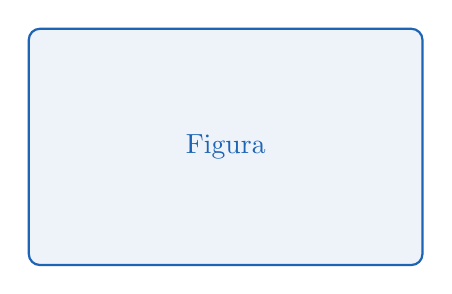
\begin{tikzpicture}
        \draw[rounded corners, thick, draw=myblue, fill=myblue!8]
          (0,0) rectangle (5,3);
        \node[text=myblue] at (2.5,1.5) {Figura};
      \end{tikzpicture}
    \end{column}
  \end{columns}
\end{frame}

% ---- animaciones ----
\begin{frame}{Animaciones}
  Revelado estándar con \texttt{[<+->]}:
  \begin{itemize}[<+->]
    \item Primero esto.
    \item Después esto.
    \item Y al final esto.
  \end{itemize}
\end{frame}

% ---- cierre ----
\begin{frame}
  \centering
  {\Large \textbf{Gracias}}
\end{frame}

\end{document}
